\documentclass{article}

\usepackage{ctex}
\usepackage[linesnumbered,ruled,vlined]{algorithm2e}
\usepackage{bookmark}
\usepackage{geometry}
\usepackage{float}
\usepackage{amsmath}
\usepackage{graphicx}
\usepackage{ulem}
\usepackage{wrapfig}
\usepackage{hyperref}

\pagestyle{headings}
\hypersetup{hidelinks}
\renewcommand\thesection{}
\renewcommand\thesubsection{}
% \renewcommand\thesubsubsection{\roman{subsubsection}}


\geometry{a4paper,scale=0.83}

\title{\vspace{-2cm}Problem Set 8}
\author{杨博涵 211300089}
\date{\today}

\begin{document}
\maketitle

%-----------------------------------------------------------------
\section{Problem 1}
时间复杂度为$\Theta(n)$, 下面是证明:

给出的单调栈算法中, 有如下事实:
\begin{enumerate}
    \item 第$i$个元素肯定会被PUSH入栈中.
    \item 第$i$个元素若被弹出, 则不会再次入栈.
\end{enumerate}

考虑$2-5$行的$n$次循环, 每次循环中, 花费$\Theta(1)$的时间对$while$中表达式进行计算, 结果为真时, 进行POP操作; 有且只有一次计算结果为假, 结束$while$. 此后进行$\Theta(1)$的PUSH操作. 设$while$中表达式为真的次数为$cnt$, 则算法运行时间为$n(c_{\text{计算表达式}} + c_{push}) + cnt \times (c_{\text{计算表达式}} + c_{pop})$.

由于$while$中表达式计算结果为真时, 栈顶元素被弹出, 由事实2, 第i个元素因后面的循环中第一个大于它的元素弹出后, 不会再次参加表达式计算, 因此每个元素对$cnt$的贡献至多为1, 因此, $cnt = O(n)$.

综上所述, 算法的时间复杂度为$\Theta(n) + O(n) = \Theta(n)$.

%-----------------------------------------------------------------
\section{Problem 2}

假设栈的扩张或缩小过程中, 每申请或者释放一个存储位置都要消耗$\Theta(1)$的时间, 只需检查对于有$n$个操作的序列, 算法运行时间复杂度是否为$O(n)$.

\subsection{(a)}

举一反例使得算法对特定操作序列复杂度为$O(n^2)$: 设$K$为2的整数次幂, 令$n = \frac{K}{2}$, 构造操作序列:
$$
\underbrace{PUSH, \cdots, PUSH}_{n-1\text{次}}, \underbrace{PUSH, POP, \cdots, PUSH, POP}_{\frac{n}{2} \text{组}PUSH, POP}
$$

设前$n-1$次操作用时$T$, 此时栈内共有$2^i - 1$个元素, 再PUSH一个元素, 栈发生扩张, 花费$\Theta(n)$的时间申请$n$个存储位置, 此时状态为$2n$个位置中$n$个位置被占用, 紧接着进行POP, 满足缩减的条件, 花费$\Theta(n)$的时间释放$n$个存储位置, 此时状态为$n$个存储位置中$n-1$个被占用. 由此, $\frac{n}{2}$组(PUSH, POP)操作中, 每一组都花费$\Theta(n)$, 因此时间复杂度为$\Theta(n^2) + T > O(n)$, 不满足条件.

\subsection{(b)}

使用核算法证明单个栈操作具有常数复杂度.

\begin{table}[H]
    \centering
    \begin{tabular}{ccc}
    \hline
     & 实际代价 & 摊还代价 \\ \hline
    PUSH & 1 & 3 \\
    POP & 1 & 3 \\
    申请或释放1个位置 & 1 & 0 \\ \hline
    \end{tabular}
    \end{table}

当栈操作未触发栈的扩张与缩减, 将差额2存入信用(初始为0)中; 否则:

\begin{description}
    \item[栈大小$n \rightarrow 2n$] 如果上一次栈发生大小变化为$\frac{n}{2} \rightarrow n$, 则有$\frac{n}{2}$的元素的差额未被使用, 信用中至少有$\frac{n}{2} \times 2 = n$的余额, 足够支付申请$n$个位置的实际代价; 如果上一次栈发生大小变化为$4n \rightarrow n$, 进一步考虑有效的差额, 如果再上一次栈的变化为$16n \rightarrow 4n$, 则有$3n$个元素的差额未被使用, $3n \times 2 > n$, 如果再上一次栈的变化为$2n \rightarrow 4n$, 则有$2n-n$个元素的差额未被使用, $n\times 2 > n$, 信用充足.
    \item[栈大小$4n \rightarrow n$] 如果上一次栈发生大小变化为$2n \rightarrow 4n$, 则有$2n$个元素的差额未被使用, $2n \times 2 > 3n$信用充足; 如果上一次栈发生大小变化为$16n \rightarrow 4n$, 进一步考虑有效的差额, 如果再上一次栈的变化为$64n \rightarrow 16n$, 则有$12n$个元素的差额未被使用, $12n \times 2 > 3n$, 如果再上一次栈的变化为$8n \rightarrow 16n$, 则有$8n-4n$个元素的差额未被使用, $4n\times 2 > 3n$, 信用充足.
\end{description}

综上所述, 任何栈操作都不会使信用变为负值, 因此单个栈操作的时间复杂度为常数.

\subsection{(c)}

使用(b)中的核算法.

\begin{description}
    \item[栈大小$n \rightarrow 2n$] 如果上一次栈发生大小变化为$\frac{n}{2} \rightarrow n$, 则有$\frac{n}{2}$的元素的差额未被使用, 信用中至少有$\frac{n}{2} \times 2 = n$的余额, 足够支付申请$n$个位置的实际代价; 如果上一次栈发生大小变化为$2n \rightarrow n$, 进一步考虑有效的差额, 如果再上一次栈的变化为$4n \rightarrow 2n$, 则有$3n$个元素的差额未被使用, $3n \times 2 > 2n$, 如果再上一次栈的变化为$2n \rightarrow 4n$, 则有$2n-n$个元素的差额未被使用, $n\times 2 > n$, 信用充足.
    \item[栈大小$2n \rightarrow n$] 如果上一次栈发生大小变化为$2n \rightarrow 4n$, 则有$2n$个元素的差额未被使用, $2n \times 2 > n$信用充足; 如果上一次栈发生大小变化为$4n \rightarrow 2n$, 进一步考虑有效的差额, 如果再上一次栈的变化为$8n \rightarrow 4n$, 则有$2n$个元素的差额未被使用, $2n \times 2 > n$, 如果再上一次栈的变化为$2n \rightarrow 4n$, 则有$n$个元素的差额未被使用, $n\times 2 > n$, 信用充足.
\end{description}

综上所述, 任何栈操作都不会使信用变为负值, 因此单个栈操作的时间复杂度为常数.

%-----------------------------------------------------------------
\section{Problem 3}

\subsection{(a)}

为了使任意一个节点的左右子树大小的差最小, 设题目中描述的以$x$为根的子树为$T$, 树的大小为$n = x.size$, 将$T$的中序遍历结果存入数组中, 数组大小为$O(n)$, 根据中序遍历数组递归地构建树: 将当前区间$[L, R]$的中点$mid$作为当前子树的根, 将左侧的点作为左子树, 右侧的点作为右子树, 递归地讨论$[L, mid - 1]$和$[mid + 1, R]$. 这种建树方式不改变中序遍历的结果, 且得到任意节点左右子树大小差值不超过1的树, 对区间$[1, n]$进行递归步骤, 即可将$T$重构为$\frac{1}{2}$-balanced tree.

上述过程中, 中序遍历用时$O(n)$, 递归建树时间$T(n) = 2T(\frac{n}{2}) + 1$, 其中1为计算中点的时间, 由主方法知$T(n) = O(n)$, 故算法时间复杂度为$O(n)$.

\subsection{(b)}

搜索用时的上界与树的高度呈线性关系, 因此只需证明$n$-node $\alpha$-balanced tree的高度为$O(\lg n)$即可.

为讨论树的高度的上界, 需要满足树的某一枝尽可能长, 而父结点与子节点子树的大小至少以$min(\alpha, 1 - \alpha)$的比例缩小, 因此构建这样一棵$n$-node $\alpha$-balanced tree: 对于树上任意节点$x$, 其左子树大小为$\alpha \cdot x.size$, 右子树大小为$(1 - \alpha) \cdot x.size$, 由已知, $\alpha \ge 1 - \alpha$, 相当于尽可能向左子树倾斜, 使得最左侧的一枝尽可能长. 此时向最左侧的一枝添加节点会破坏$\alpha$平衡的性质, 故树的最大高度为$\log_{\alpha^{-1}} n = O(\lg n)$, 原命题成立.

\subsection{(c)}

根据题目中的定义, 任意BST的势=与$\alpha$有关的非负常数$\times \ \ k$个大于1的正数的和, 其中$k \ge 0$, 因此势非负.

$\frac{1}{2}$-balanced tree中, 任意$x$有$\Delta x \le 1$(当且仅当$x$左右子树大小为奇数时$\Delta x = 1$), 因此:
$$
\left(\sum_{x \in T: \Delta(x) \geq 2} \Delta(x)\right) = 0
$$

综上所述, $\frac{1}{2}$-balanced tree的势为0.

\subsection{(d)}

问题中假定$m$个单位的势够支付重建$m$结点子树的代价, 重建的结果是势为0的$\frac{1}{2}$-balanced tree:
$$
\sum_{i=1}^n \hat{c}_i=\sum_{i=1}^n\left(c_i+\Phi\left(D_i\right)-\Phi\left(D_{i-1}\right)\right)=\sum_{i=1}^n c_i+\Phi\left(D_n\right)-\Phi\left(D_0\right) = \sum_{i=1}^n c_i - \Phi\left(D_0\right) $$

说明$\Phi\left(D_0\right)$至少为$m$, 才能支付足够的势, 记$sum(\Delta) = \sum_{x \in T: \Delta(x) \geq 2} \Delta(x)$, 有$c \ge \dfrac{m}{sum(\Delta)}$, 因此当$sum(\Delta)$取最小值时, 仍满足不等式的$c$即为所求.

对于根为$x$的大小为m的子树$T$, 若只有$x$节点不满足$\alpha$-平衡, 而其余节点皆满足$\alpha$-平衡, 并且$\Delta(x)$有最小值, 则此时$sum(\Delta)$取最小值, 其值为$\alpha m - (1 - \alpha)m = (2\alpha - 1)m$, 代入, 得$c \ge \dfrac{1}{2\alpha - 1}$.

\subsection{(e)}

(b)证明搜索一个点用时$O(\lg n)$, 则在插入或者删除的过程中, 首先搜索找到指定位置用时$O(\lg n)$, 并且在搜索过程中经过的路径有$O(\lg n)$个节点. 由于节点的插入或删除可能其祖先不再$\alpha$-平衡, 因此在回溯的过程中还要通过rebuild维护, 而目标节点的祖先有$O(\lg n)$个, 从最深的祖先开始维护, 每个不平衡节点用时$O(1)$, 故维护用时为$O(\lg n)$, 综上所述, 单次插入或删除的摊还时间为$O(\lg n)$.

%-----------------------------------------------------------------
\section{Problem 4}

Professor F. Lake的想法是可行的, 将让每个集合链表中的末尾作为该集合的代表, 链表中每个元素分别指向链表末尾以及后继, 每个集合保存链表的head, 即可实现与原来相同复杂度的操作.

\begin{description}
    \item[MAKE-SET(x)] 只需建立只有一个指针的链表, 并将head指向代表$x$节点, 时间复杂度为$O(1)$, 与原来的复杂度相同.
    \item[FIND-SET(x)] 由于集合中链表上每个结点都有指向链表末尾的指针, 而此时链表末尾作为该集合的代表, 因此只需$O(1)$的指针访问, 与原来的复杂度相同.
    \item[UNION(x, y)] 仍然使用加权合井的启发式策略, 将较小的集合合并入较大的集合, 具体操作方式是将较短的链表连接在较长链表之前, 获取较大集合的head属性, 将较短链表的末尾的后继指向head, 然后更新短链表中指向末尾的指针, 最后使用较小集合的head作为合并后的集合的head. 如下图所示:
    \begin{figure}[H]
        \centering
        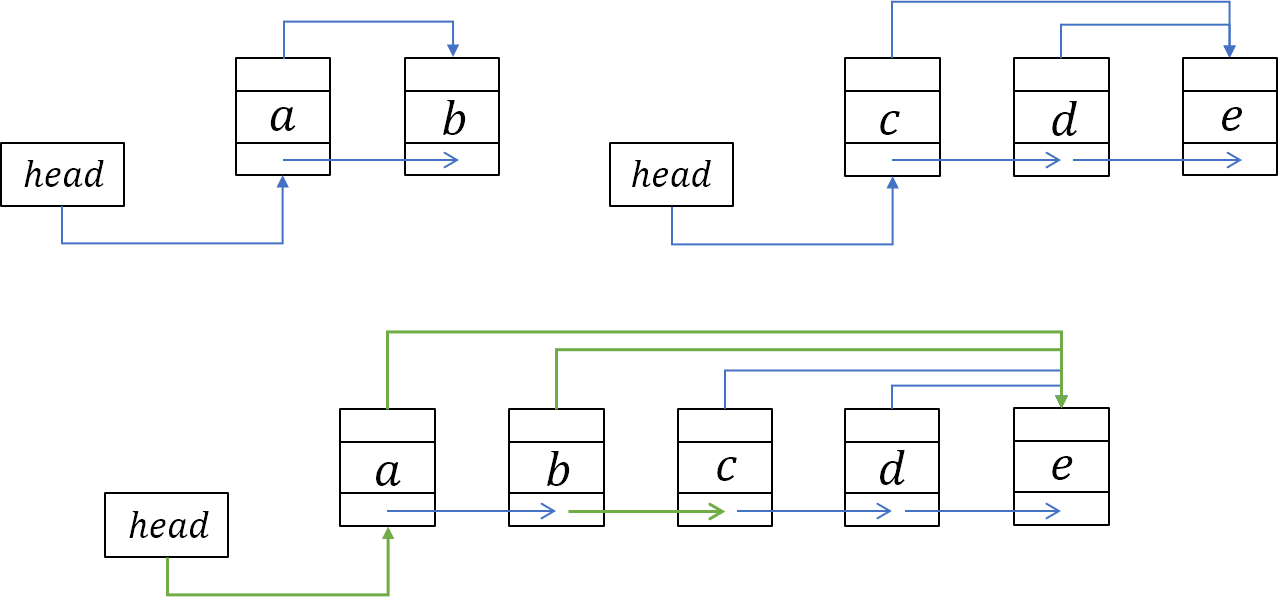
\includegraphics[width=0.7\textwidth]{1.png}
    \end{figure}
    保证了每次合并的复杂度取决于较小集合的大小, 如果两个集合都有$\Omega (n)$个成员, 则单个的UNION操作仍然需要$\Omega (n)$的时间。与原来的复杂度相同.
\end{description}

%-----------------------------------------------------------------
\section{Problem 5}

为树中每个节点添加一个$.next$后继属性, 形成一个由树中节点构成的链表, 这个链表首尾相接形成一个环, 即可实现与原来相同复杂度的操作, 而且打印一棵有$n$个节点的树用时$\Theta(n)$.

\begin{description}
    \item[MAKE-SET(x)] 建立只有根节点的树, 其后继即为自身, 形成一个自环, 时间复杂度$O(1)$.
    \item[FIND-SET(x)] 此操作不会影响树的对应链表, 因此实现与原来操作完全相同.
    \item[UNION(x, y)] 启发式合并策略不变, 假设合并过程中, 树$B$被合并到树$A$上, 考虑$B$与$A$的根节点及其后继$rt_A \rightarrow son_A, rt_B \rightarrow son_B$, 将两棵子树对应的环打开, 重新设置后继为$rt_B \rightarrow son_A, rt_A \rightarrow son_B$, 既将$B$打开后将$A$重新连接为一个环, 上述操作只需要4次指针访问操作, 相当于为原始操作的复杂度加上一个小常数, 渐进复杂度不变.
    \item[PRINTSET(x)] 以$x$为起点, 遍历$x$所在的环, 若$x$所在树有$n$个点, 则环上也有$n$个点, 每次循环打印$x$并访问$x$的后继, 用时为常数, 因此PRINTSET(x)时间复杂度为$\Theta(n)$, 与$x$所在树大小呈线性关系.
\end{description}

\begin{algorithm}[H]
    \caption{PRINTSET(x)}
    $start \leftarrow x$ \\
    $x \leftarrow x.next$ \\
    \While{$x \ne start$}{
        \textbf{PRINT}(x) \\
        $x \leftarrow x.next$
    }
\end{algorithm}

\end{document}